\documentclass[a4paper,12pt]{article}

\usepackage{graphicx}
\usepackage{caption}
\usepackage{subcaption}
\usepackage{tikz}
\usepackage{pgf}
\usepackage{amsmath}
\usepackage{amssymb}
\usetikzlibrary{arrows.meta}
\usepackage[utf8]{inputenc}
\usepackage[english,greek]{babel}
\usepackage[hidelinks]{hyperref}

\begin{document}
\selectlanguage{greek}

\begin{center}
    {\Large ΕΡΓΑΣΙΑ ΣΤΟ ΜΑΘΗΜΑ ΒΑΣΕΙΣ ΔΕΔΟΜΕΝΩΝ}\\[3cm]

    {\Large \selectlanguage{english}\textbf{CryptfolioDB}\selectlanguage{greek}}\\[0.5cm]

    {\large Μία προσωπική εφαρμογή επενδύσεων και παρακολούθησης κρυπτονομισμάτων }\\[3cm]

    {\Large Πρώτο Παραδοτέο}\\[3cm]

    {\large Ομάδα 39}\\[1cm]

    \begin{tabular}{l l l}
        Δασκαλόπουλος Αριστείδης & 10640 & \selectlanguage{english}\texttt{arisdask@ece.auth.gr}\selectlanguage{greek} \\
        Λαβδάκης Γεώργιος & 10672 & \selectlanguage{english}\texttt{glavdakis@ece.auth.gr}\selectlanguage{greek} \\
        Ρουσομάνης Γεώργιος & 10703 & \selectlanguage{english}\texttt{rousoman@ece.auth.gr}\selectlanguage{greek} \\
    \end{tabular}\\[3cm]

    {\large 19/11/2025}
\end{center}

\newpage

\tableofcontents

\newpage

\section{Εισαγωγή}

\subsection{Σκοπός Εφαρμογής}

Ο σκοπός της εφαρμογής \selectlanguage{english}CryptfolioDB\selectlanguage{greek} 
είναι η αποθήκευση, οργάνωση και παρακολούθηση των επενδύσεων ενός χρήστη 
σε κρυπτονομίσματα. Η βάση δεδομένων επιτρέπει την καταγραφή πορτοφολιών, 
υπολοίπων και συναλλαγών, προσφέροντας μια συγκεντρωτική εικόνα του χαρτοφυλακίου.

\subsection{Περιγραφή Εφαρμογής}

Η εφαρμογή επιτρέπει στον χρήστη να δημιουργεί και να διαχειρίζεται 
πολλαπλά ψηφιακά πορτοφόλια, να αποθηκεύει τα υπόλοιπα κάθε κρυπτονομίσματος, 
να καταχωρεί συναλλαγές και να παρακολουθεί τις διακυμάνσεις των τιμών 
μέσω των ιδιοτήτων των κρυπτονομισμάτων. 
Οι χρήστες έχουν πρόσβαση στο ιστορικό των συναλλαγών τους, 
στο προσωποποιημένο χαρτοφυλάκιό τους και σε στατιστικά στοιχεία.

\subsection{Απαιτήσεις Εφαρμογής σε Δεδομένα}

Η βάση αναμένεται να αποθηκεύει δεδομένα για όλους τους χρήστες της εφαρμογής, 
τα πορτοφόλια τους και τις αντίστοιχες συναλλαγές. 
Εκτιμάται ότι κάθε χρήστης θα διατηρεί από 1 έως 5 πορτοφόλια, 
με 20–200 συναλλαγές ανά πορτοφόλι. 
Η βάση υποστηρίζει επίσης δεδομένα για δεκάδες έως εκατοντάδες κρυπτονομίσματα, 
μαζί με τις μεταβαλλόμενες τιμές και τεχνικές πληροφορίες τους.

\newpage

\section{Κατηγορίες Χρηστών και Απαιτήσεις τους}

\subsection*{Τελικός Χρήστης}
Ο χρήστης της εφαρμογής έχει τις ακόλουθες δυνατότητες:

\begin{itemize}
    \item Δημιουργία και επεξεργασία ψηφιακών πορτοφολιών.
    \item Προσθήκη/επεξεργασία υπολοίπων κρυπτονομισμάτων.
    \item Καταγραφή συναλλαγών αγοράς, πώλησης ή μεταφοράς.
    \item Προβολή συνολικής αξίας χαρτοφυλακίου.
    \item Παρακολούθηση τιμών κρυπτονομισμάτων.
\end{itemize}

\newpage

\section{Μοντέλο Οντοτήτων/Συσχετίσεων}

\subsection{Γενική Περιγραφή}

Το σύστημα αποτελείται από τις οντότητες 
\selectlanguage{english}User, Wallet, WalletBalance, Cryptocurrency, Transaction\selectlanguage{greek}. 
Κάθε χρήστης μπορεί να διαθέτει πολλά πορτοφόλια, ενώ κάθε πορτοφόλι μπορεί να 
περιέχει υπόλοιπα για πολλά κρυπτονομίσματα. 
Οι συναλλαγές πραγματοποιούνται σε επίπεδο πορτοφολιού και 
σχετίζονται με συγκεκριμένα κρυπτονομίσματα. 

\subsubsection*{Υποθέσεις}
\begin{itemize}
    \item Το σύμβολο του κάθε κρυπτονομίσματος είναι μοναδικό 
\end{itemize}

\subsection{Καθορισμός Οντοτήτων}

% =============================
% USER
% =============================

\begin{tabular}{|p{4cm}|p{10cm}|}
\hline
\textbf{Όνομα Οντότητας} & \selectlanguage{english}User\selectlanguage{greek} \\ \hline

\textbf{Περιγραφή} & Αντιπροσωπεύει έναν εγγεγραμμένο χρήστη του συστήματος. \\ \hline

\textbf{Ιδιότητες Οντότητας} & Ισχυρή οντότητα \selectlanguage{english}(Strong Entity)\selectlanguage{greek}. 
Διαθέτει πρωτεύον κλειδί. \\ \hline

\textbf{Γνωρίσματα} &
\begin{itemize}
    \item \selectlanguage{english}email (PK)\selectlanguage{greek}: Η μοναδική διεύθυνση \selectlanguage{english}
    email\selectlanguage{greek}.
    \item \selectlanguage{english}name\selectlanguage{greek}: Το όνομα χρήστη.
\end{itemize}
\\ \hline
\end{tabular}

\vspace{1cm}

% =============================
% WALLET
% =============================

\begin{tabular}{|p{4cm}|p{10cm}|}
\hline
\textbf{Όνομα Οντότητας} & \selectlanguage{english}Wallet\selectlanguage{greek} \\ \hline

\textbf{Περιγραφή} & Ψηφιακό πορτοφόλι που ανήκει σε έναν χρήστη. \\ \hline

\textbf{Ιδιότητες Οντότητας} & Ισχυρή οντότητα \selectlanguage{english}(Strong Entity)\selectlanguage{greek}. 
Συνδέεται με χρήστη ως εξαρτώμενη αλλά όχι ασθενής. \\ \hline

\textbf{Γνωρίσματα} &
\begin{itemize}
    \item \selectlanguage{english}walletID (PK)\selectlanguage{greek}: Μοναδικό αναγνωριστικό πορτοφολιού.
    \item \selectlanguage{english}walletName\selectlanguage{greek}: Όνομα του πορτοφολιού.
    \item \selectlanguage{english}walletType\selectlanguage{greek}: Τύπος (π.χ. \selectlanguage{english}Spot, 
    Futures\selectlanguage{greek}).
\end{itemize}
\\ \hline
\end{tabular}

\vspace{1cm}

% =============================
% WALLET BALANCE
% =============================

\begin{tabular}{|p{4cm}|p{10cm}|}
\hline
\textbf{Όνομα Οντότητας} & \selectlanguage{english}WalletBalance\selectlanguage{greek} \\ \hline

\textbf{Περιγραφή} & Καταγράφει το διαθέσιμο υπόλοιπο κάθε κρυπτονομίσματος σε κάθε πορτοφόλι. \\ \hline

\textbf{Ιδιότητες Οντότητας} & Ασθενής οντότητα \selectlanguage{english}(Weak Entity)\selectlanguage{greek}. 
Εξαρτάται από τα \selectlanguage{english}Wallet\selectlanguage{greek} και \selectlanguage{english}Cryptocurrency
\selectlanguage{greek}. \\ \hline

\textbf{Γνωρίσματα} &
\begin{itemize}
    \item \selectlanguage{english}amount\selectlanguage{greek}: Υπόλοιπο.
    \item \selectlanguage{english}lastUpdated\selectlanguage{greek}: Τελευταία ενημέρωση.
\end{itemize}
\\ \hline
\end{tabular}

\vspace{1cm}

% =============================
% CRYPTOCURRENCY
% =============================

\begin{tabular}{|p{4cm}|p{10cm}|}
\hline
\textbf{Όνομα Οντότητας} & \selectlanguage{english}Cryptocurrency\selectlanguage{greek} \\ \hline

\textbf{Περιγραφή} & Πληροφορίες για κάθε υποστηριζόμενο κρυπτονόμισμα. \\ \hline

\textbf{Ιδιότητες Οντότητας} & Ισχυρή οντότητα \selectlanguage{english}(Strong Entity)\selectlanguage{greek}. 
Το \selectlanguage{english}symbol\selectlanguage{greek} αποτελεί φυσικό πρωτεύον κλειδί. \\ \hline

\textbf{Γνωρίσματα} &
\begin{itemize}
    \item \selectlanguage{english}symbol (PK)\selectlanguage{greek}: Π.χ. \selectlanguage{english}BTC, 
    ETH\selectlanguage{greek}.
    \item \selectlanguage{english}marketCap\selectlanguage{greek}: 
    Η αξία του κρυπτονομίσματος στην αγορά.
    \item \selectlanguage{english}circulatingSupply\selectlanguage{greek}: 
    Ο αριθμός νομισμάτων που κυκλοφορούν.

\end{itemize}
\\ \hline
\end{tabular}

\vspace{1cm}

% =============================
% TRANSACTION
% =============================

\begin{tabular}{|p{4cm}|p{10cm}|}
\hline
\textbf{Όνομα Οντότητας} & \selectlanguage{english}Transaction\selectlanguage{greek} \\ \hline

\textbf{Περιγραφή} & Μια συναλλαγή που πραγματοποιείται σε συγκεκριμένο πορτοφόλι. \\ \hline

\textbf{Ιδιότητες Οντότητας} & Ισχυρή οντότητα \selectlanguage{english}(Strong Entity)\selectlanguage{greek}
με δικό της πρωτεύον κλειδί. \\ \hline

\textbf{Γνωρίσματα} &
\begin{itemize}
    \item \selectlanguage{english}transactionID (PK)\selectlanguage{greek}: Αναγνωριστικό συναλλαγής.
    \item \selectlanguage{english}amount\selectlanguage{greek}: Ποσό συναλλαγής.
    \item \selectlanguage{english}transactionType\selectlanguage{greek}: Τύπος \selectlanguage{english}
    (Deposit, Withdrawal, Trade)\selectlanguage{greek}.
    \item \selectlanguage{english}timestamp\selectlanguage{greek}: Χρονική σήμανση.
    \item \selectlanguage{english}priceAtTimestamp\selectlanguage{greek}: Η τιμή του κρυπτονομίσματος κατά την 
    συναλλαγή
\end{itemize}
\\ \hline
\end{tabular}


\textbf{Συσχέτιση 1:} \selectlanguage{english}User\_Owns\_Wallet\selectlanguage{greek}

\textbf{Περιγραφή:} Κάθε χρήστης διαθέτει ένα ή περισσότερα πορτοφόλια.

\textbf{Ιδιότητες:} Συσχέτιση τύπου 1:N.

\textbf{Πληθικότητα:} 
\selectlanguage{english}User (1) -- (N) Wallet\selectlanguage{greek}.

\bigskip

\textbf{Συσχέτιση 2:} \selectlanguage{english}Wallet\_Has\_Balance\selectlanguage{greek}

\textbf{Περιγραφή:} Κάθε πορτοφόλι μπορεί να περιέχει υπόλοιπα πολλών κρυπτονομισμάτων.

\textbf{Ιδιότητες:} Συσχέτιση τύπου N:N μέσω της ασθενούς οντότητας 
\selectlanguage{english}WalletBalance\selectlanguage{greek}.

\textbf{Πληθικότητα:} 
\selectlanguage{english}Wallet (1) -- (N) WalletBalance (N) -- (1) Cryptocurrency\selectlanguage{greek}.

\bigskip

\textbf{Συσχέτιση 3:} \selectlanguage{english}Wallet\_Has\_Transaction\selectlanguage{greek}

\textbf{Περιγραφή:} Κάθε συναλλαγή ανήκει σε ένα συγκεκριμένο πορτοφόλι.

\textbf{Ιδιότητες:} Συσχέτιση 1:N.

\textbf{Πληθικότητα:} 
\selectlanguage{english}Wallet (1) -- (N) Transaction\selectlanguage{greek}.

\bigskip

\textbf{Συσχέτιση 4:} \selectlanguage{english}Transaction\_Involves\_Cryptocurrency\selectlanguage{greek}

\textbf{Περιγραφή:} Κάθε συναλλαγή αφορά ένα και μόνο ένα κρυπτονόμισμα.

\textbf{Ιδιότητες:} Συσχέτιση 1:N.

\textbf{Πληθικότητα:} 
\selectlanguage{english}Cryptocurrency (1) -- (N) Transaction\selectlanguage{greek}.


\subsection{Διάγραμμα Οντοτήτων/Συσχετίσεων}

\begin{figure}[h]
    \centering
    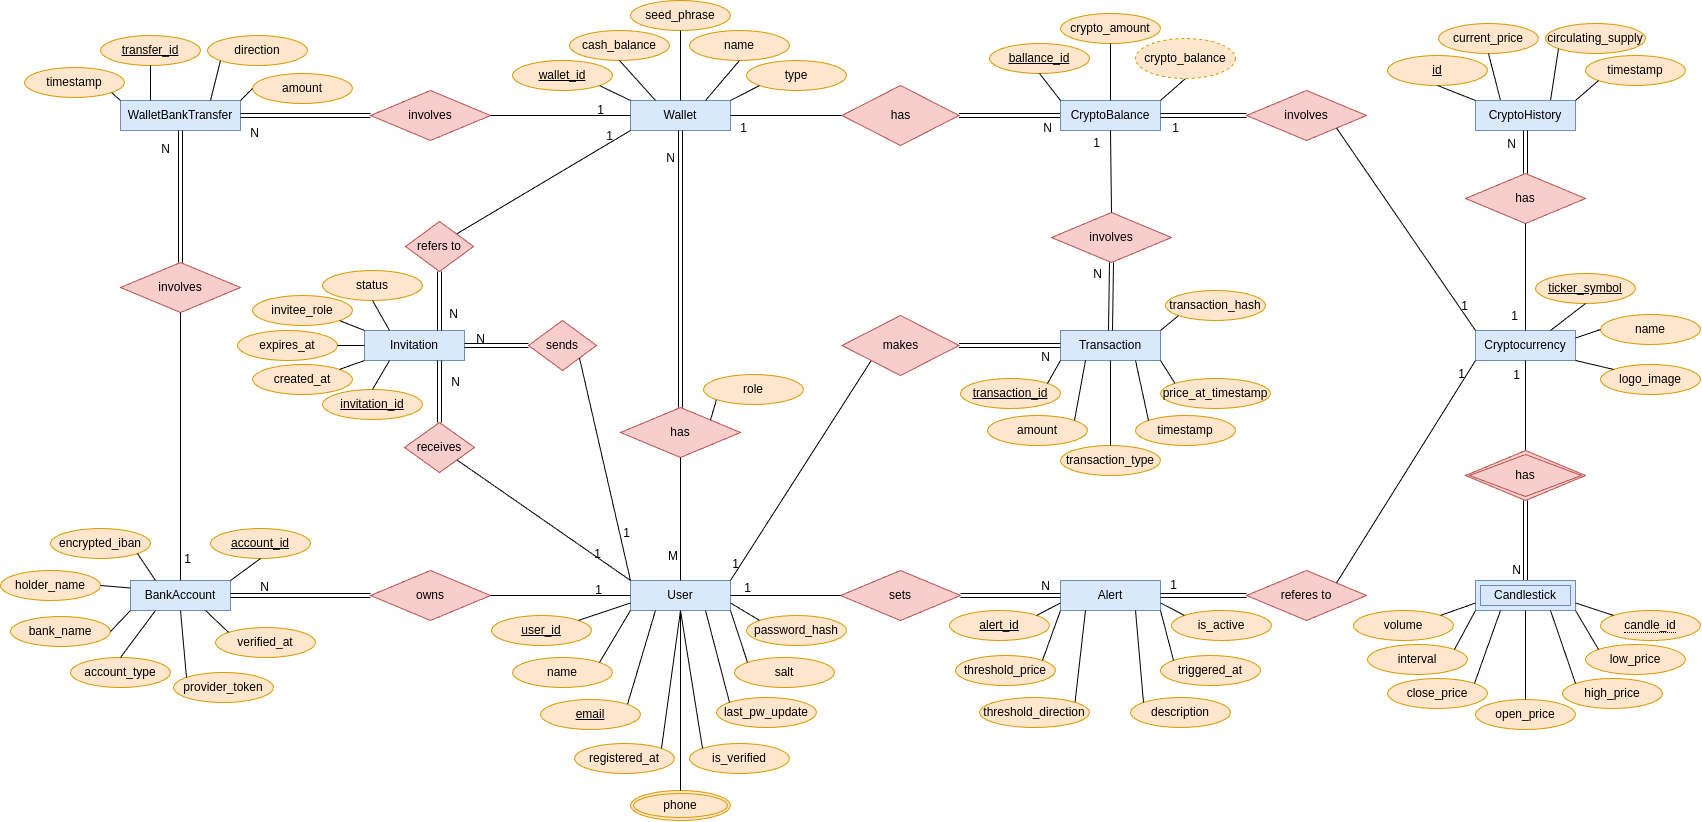
\includegraphics[width=1\linewidth]{ER_diagram.png}
    \label{fig:ER}
\end{figure}
\newpage

\section{Σχεσιακό Μοντέλο}

\subsection{Πεδία Ορισμού}

\begin{tabular}{|p{6cm}|p{6cm}|}
\hline
\textbf{Πεδίο Ορισμού} & \textbf{Τύπος} \\ \hline

Όνομα & \selectlanguage{english}VARCHAR(30) \\ \hline
Μικρό Αλφαριθμητικό & \selectlanguage{english}VARCHAR(20) \\ \hline
Μεσαίο Αλφαριθμητικό & \selectlanguage{english}VARCHAR(50) \\ \hline
Απλό Αλφαριθμητικό & \selectlanguage{english}VARCHAR(150) \\ \hline
Κρυπτογραφημένο & \selectlanguage{english}VARCHAR(512) \\ \hline
Ακέραιος & \selectlanguage{english}INTEGER \\ \hline
Αναγνωριστικό & \selectlanguage{english}SERIAL \\ \hline
Κείμενο & \selectlanguage{english}TEXT \\ \hline
Δεκαδικός & \selectlanguage{english}DECIMAL(18,2) \\ \hline
Δεκαδικός Υψηλής Ακρίβειας & \selectlanguage{english}DECIMAL(18,8) \\ \hline
Μεγάλος Δεκαδικός & \selectlanguage{english}DECIMAL(30,2) \\ \hline
Ημερομηνία και Ώρα & \selectlanguage{english}DATETIME \\ \hline
Λογική Τιμή & \selectlanguage{english}BOOLEAN \\ \hline
Αρχείο Εικόνας & \selectlanguage{english}BLOB \\ \hline

\end{tabular}

\newpage

\subsection{Σχέσεις}

\begin{tabular}{|p{6cm}|p{6cm}|}
\hline
\textbf{Όνομα Σχέσης} & \selectlanguage{english}User \\ \hline

\multicolumn{2}{|l|}{\textbf{Γνωρίσματα:}} \\ \hline
\selectlanguage{english}user\_id & Αναγνωριστικό \\ \hline
\selectlanguage{english}name & Όνομα \\ \hline
\selectlanguage{english}email & Απλό Αλφαριθμητικό \\ \hline
\selectlanguage{english}registered\_at & Ημερομηνία και Ώρα \\ \hline
\selectlanguage{english}phone & Μεσαίο Αλφαριθμητικό \\ \hline
\selectlanguage{english}is\_verified & Λογική Τιμή \\ \hline
\selectlanguage{english}last\_pw\_update & Ημερομηνία και Ώρα \\ \hline
\selectlanguage{english}password\_hash & Κείμενο \\ \hline
\selectlanguage{english}salt & Κείμενο \\ \hline

\multicolumn{2}{|l|}{\textbf{Περιορισμοί Ακεραιότητας:}} \\ \hline
Πρωτεύον Κλειδί & \selectlanguage{english}user\_id, email \\ \hline
Ξένα Κλειδιά & - \\ \hline
\end{tabular}

\newpage

\begin{tabular}{|p{6cm}|p{6cm}|}
\hline
\textbf{Όνομα Σχέσης} & \selectlanguage{english}Wallet \\ \hline

\multicolumn{2}{|l|}{\textbf{Γνωρίσματα:}} \\ \hline
\selectlanguage{english}wallet\_id & Αναγνωριστικό \\ \hline
\selectlanguage{english}cash\_balance & Δεκαδικός \\ \hline
\selectlanguage{english}seed\_phrase & Κείμενο \\ \hline
\selectlanguage{english}name & Όνομα \\ \hline
\selectlanguage{english}type & Μικρό Αλφαριθμητικό \\ \hline

\multicolumn{2}{|l|}{\textbf{Περιορισμοί Ακεραιότητας:}} \\ \hline
Πρωτεύον Κλειδί & \selectlanguage{english}wallet\_id \\ \hline
Ξένα Κλειδιά & - \\ \hline
\end{tabular}

\vspace{1cm}

\begin{tabular}{|p{6cm}|p{6cm}|}
\hline
\textbf{Όνομα Σχέσης} & \selectlanguage{english}BankAccount \\ \hline

\multicolumn{2}{|l|}{\textbf{Γνωρίσματα:}} \\ \hline
\selectlanguage{english}account\_id & Αναγνωριστικό \\ \hline
\selectlanguage{english}encrypted\_iban & Κρυπτογραφημένο \\ \hline
\selectlanguage{english}holder\_name & Όνομα \\ \hline
\selectlanguage{english}bank\_name & Απλό Αλφαριθμητικό \\ \hline
\selectlanguage{english}account\_type & Απλό Αλφαριθμητικό \\ \hline
\selectlanguage{english}provider\_token & Κείμενο \\ \hline
\selectlanguage{english}verified\_at & Ημερομηνία και Ώρα \\ \hline
\selectlanguage{english}user\_id & Αναγνωριστικό \\ \hline

\multicolumn{2}{|l|}{\textbf{Περιορισμοί Ακεραιότητας:}} \\ \hline
Πρωτεύον Κλειδί & \selectlanguage{english}account\_id \\ \hline
Ξένα Κλειδιά & \selectlanguage{english}user\_id User to BankAccount \\ \hline
\end{tabular}

\vspace{1cm}

\begin{tabular}{|p{6cm}|p{6cm}|}
\hline
\textbf{Όνομα Σχέσης} &\selectlanguage{english} WalletBankTransfer \\ \hline

\multicolumn{2}{|l|}{\textbf{Γνωρίσματα:}} \\ \hline
\selectlanguage{english}transfer\_id & Αναγνωριστικό \\ \hline
\selectlanguage{english}amount & Δεκαδικός \\ \hline
\selectlanguage{english}direction & Μικρό Αλφαριθμητικό \\ \hline
\selectlanguage{english}timestamp & Ημερομηνία και Ώρα \\ \hline
\selectlanguage{english}wallet\_id & Αναγνωριστικό \\ \hline
\selectlanguage{english}account\_id & Ακέραιος \\ \hline

\multicolumn{2}{|l|}{\textbf{Περιορισμοί Ακεραιότητας:}} \\ \hline
Πρωτεύον Κλειδί & \selectlanguage{english}transfer\_id \\ \hline
Ξένα Κλειδιά & \{\selectlanguage{english}wallet\_id 

Wallet to WalletBankTransfer, \selectlanguage{english}account\_id BankAccount to 

WalletBankTransfer\} \\ \hline
\end{tabular}

\vspace{1cm}

\begin{tabular}{|p{6cm}|p{6cm}|}
\hline
\textbf{Όνομα Σχέσης} & \selectlanguage{english}Transaction \\ \hline

\multicolumn{2}{|l|}{\textbf{Γνωρίσματα:}} \\ \hline
\selectlanguage{english}transaction\_id & Αναγνωριστικό \\ \hline
\selectlanguage{english}amount & Δεκαδικός \\ \hline
\selectlanguage{english}transaction\_type & Μικρό Αλφαριθμητικό \\ \hline
\selectlanguage{english}timestamp & Ημερομηνία και Ώρα \\ \hline
\selectlanguage{english}price\_at\_timestamp & Δεκαδικός Υψηλής Ακρίβειας \\ \hline
\selectlanguage{english}transaction\_type & Κείμενο \\ \hline
\selectlanguage{english}user\_id & Αναγνωριστικό \\ \hline
\selectlanguage{english}balance\_id & Αναγνωριστικό \\ \hline

\multicolumn{2}{|l|}{\textbf{Περιορισμοί Ακεραιότητας:}} \\ \hline
Πρωτεύον Κλειδί & \selectlanguage{english}transaction\_id \\ \hline
Ξένα Κλειδιά & \{\selectlanguage{english}user\_id User to Transaction,

balance\_id CryproBallance to Transaction\} \\ \hline
\end{tabular}

\vspace{1cm}

\begin{tabular}{|p{6cm}|p{6cm}|}
\hline
\textbf{Όνομα Σχέσης} & \selectlanguage{english}Invitation \\ \hline

\multicolumn{2}{|l|}{\textbf{Γνωρίσματα:}} \\ \hline
\selectlanguage{english}invitation\_id & Αναγνωριστικό \\ \hline
\selectlanguage{english}status & Μικρό Αλφαριθμητικό \\ \hline
\selectlanguage{english}created\_at & Ημερομηνία και Ώρα \\ \hline
\selectlanguage{english}expires\_at & Ημερομηνία και Ώρα \\ \hline
\selectlanguage{english}invitee\_role & Μικρό Αλφαριθμητικό \\ \hline
\selectlanguage{english}inviter\_id & Αναγνωριστικό \\ \hline
\selectlanguage{english}invitee\_id & Αναγνωριστικό \\ \hline
\selectlanguage{english}wallet\_id & Αναγνωριστικό \\ \hline

\multicolumn{2}{|l|}{\textbf{Περιορισμοί Ακεραιότητας:}} \\ \hline
Πρωτεύον Κλειδί & \selectlanguage{english}invitation\_id \\ \hline
Ξένα Κλειδιά & \{\selectlanguage{english}inviter\_id User to Invitation, 

invitee\_id User to Invitation, 

wallet\_id Wallet to Invitation\} \\ \hline
\end{tabular}

\vspace{1cm}

\begin{tabular}{|p{6cm}|p{6cm}|}
\hline
\textbf{Όνομα Σχέσης} & \selectlanguage{english}Alert \\ \hline

\multicolumn{2}{|l|}{\textbf{Γνωρίσματα:}} \\ \hline
\selectlanguage{english}alert\_id & Αναγνωριστικό \\ \hline
\selectlanguage{english}threshold\_price & Δεκαδικός Υψηλής Ακρίβειας \\ \hline
\selectlanguage{english}threshold\_direction & Μικρό Αλφαριθμητικό \\ \hline
\selectlanguage{english}description & Κείμενο \\ \hline
\selectlanguage{english}is\_active & Λογική Τιμή \\ \hline
\selectlanguage{english}triggered\_at & Ημερομηνία και Ώρα \\ \hline
\selectlanguage{english}user\_id & Ακέραιος \\ \hline
\selectlanguage{english}ticker\_symbol & Μικρό Αλφαριθμητικό \\ \hline

\multicolumn{2}{|l|}{\textbf{Περιορισμοί Ακεραιότητας:}} \\ \hline
Πρωτεύον Κλειδί & \selectlanguage{english}alert\_id \\ \hline
Ξένα Κλειδιά & \{\selectlanguage{english}email User to Alert,   

\selectlanguage{english}ticker\_symbol Cryptocurrency to Alert\} \\ \hline
\end{tabular}

\vspace{1cm}

\begin{tabular}{|p{6cm}|p{6cm}|}
\hline
\textbf{Όνομα Σχέσης} & \selectlanguage{english}Cryptocurrency \\ \hline

\multicolumn{2}{|l|}{\textbf{Γνωρίσματα:}} \\ \hline
\selectlanguage{english}ticker\_symbol & Μικρό Αλφαριθμητικό \\ \hline
\selectlanguage{english}name & Όνομα \\ \hline
\selectlanguage{english}logo\_image & Αρχείο Εικόνας \\ \hline

\multicolumn{2}{|l|}{\textbf{Περιορισμοί Ακεραιότητας:}} \\ \hline
Πρωτεύον Κλειδί & \selectlanguage{english}ticker\_symbol \\ \hline
Ξένα Κλειδιά & - \\ \hline
\end{tabular}

\vspace{1cm}

\begin{tabular}{|p{6cm}|p{6cm}|}
\hline
\textbf{Όνομα Σχέσης} & \selectlanguage{english}Candlestick \\ \hline

\multicolumn{2}{|l|}{\textbf{Γνωρίσματα:}} \\ \hline
\selectlanguage{english}candle\_id & Αναγνωριστικό \\ \hline
\selectlanguage{english}low\_price & Δεκαδικός Υψηλής Ακρίβειας \\ \hline
\selectlanguage{english}high\_price & Δεκαδικός Υψηλής Ακρίβειας \\ \hline
\selectlanguage{english}open\_price & Δεκαδικός Υψηλής Ακρίβειας \\ \hline
\selectlanguage{english}close\_price & Δεκαδικός Υψηλής Ακρίβειας \\ \hline
\selectlanguage{english}volume & Μεγάλος Δεκαδικός \\ \hline
\selectlanguage{english}interval & Μικρό Αλφαριθμητικό \\ \hline
\selectlanguage{english}ticker\_symbol & Μικρό Αλφαριθμητικό \\ \hline

\multicolumn{2}{|l|}{\textbf{Περιορισμοί Ακεραιότητας:}} \\ \hline
Πρωτεύον Κλειδί & \selectlanguage{english}candle\_id \\ \hline
Ξένα Κλειδιά & \selectlanguage{english}ticker\_symbol Cryptocurrency to Candlestick\\ \hline
\end{tabular}

\vspace{1cm}

\begin{tabular}{|p{6cm}|p{6cm}|}
\hline
\textbf{Όνομα Σχέσης} & \selectlanguage{english}CryptoBalance \\ \hline

\multicolumn{2}{|l|}{\textbf{Γνωρίσματα:}} \\ \hline
\selectlanguage{english}balance\_id &  Αναγνωριστικό \\ \hline
\selectlanguage{english}crypto\_amount & Ακέραιος \\ \hline
\selectlanguage{english}crypto\_balance & Μεγάλος Δεκαδικός \\ \hline
\selectlanguage{english}wallet\_id & Αναγνωριστικό \\ \hline
\selectlanguage{english}ticker\_symbol & Μικρό Αλφαριθμητικό \\ \hline

\multicolumn{2}{|l|}{\textbf{Περιορισμοί Ακεραιότητας:}} \\ \hline
Πρωτεύον Κλειδί & \selectlanguage{english}balance\_id \\ \hline
Ξένα Κλειδιά & \{\selectlanguage{english}ticker\_symbol Cryptocurrency to CryptoBalance, wallet\_id Wallet to CryptoBalance\} \\ \hline
\end{tabular}

\vspace{1cm}

\begin{tabular}{|p{6cm}|p{6cm}|}
\hline
\textbf{Όνομα Σχέσης} & \selectlanguage{english}CryptoHistory \\ \hline

\multicolumn{2}{|l|}{\textbf{Γνωρίσματα:}} \\ \hline
\selectlanguage{english}id & Αναγνωριστικό \\ \hline
\selectlanguage{english}current\_price & Μεγάλος Δεκαδικός \\ \hline
\selectlanguage{english}circulating\_supply & Μεγάλος Δεκαδικός \\ \hline
\selectlanguage{english}timestamp & Ημερομηνία και ΄Ωρα \\ \hline
\selectlanguage{english}ticker\_symbol & Μικρό Αλφαριθμητικό \\ \hline

\multicolumn{2}{|l|}{\textbf{Περιορισμοί Ακεραιότητας:}} \\ \hline
Πρωτεύον Κλειδί & \selectlanguage{english}id \\ \hline
Ξένα Κλειδιά & \selectlanguage{english}ticker\_symbol Cryptocurrency to CryptoHistory\\ \hline
\end{tabular}

\newpage

\subsection{Σχεσιακό Σχήμα}






\subsection{Όψεις}

\begin{flushleft}
1) Όψη για τον αριθμό \selectlanguage{english}crypto\selectlanguage{greek} των χρηστών

\begin{figure}[h]
    \centering
    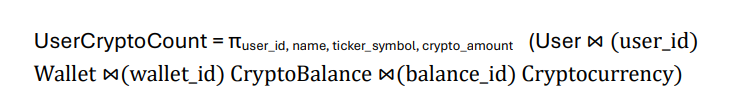
\includegraphics[width=0.8\linewidth]{view1.png}
    \label{fig:placeholder}
\end{figure}

2) Όψη για τις συναλλαγές \selectlanguage{english}crypto\selectlanguage{greek} των χρηστών

\begin{figure}[h]
    \centering
    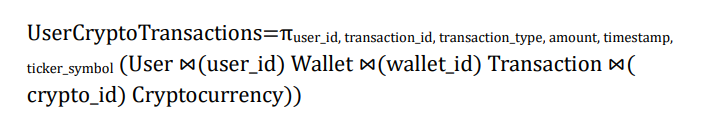
\includegraphics[width=0.8\linewidth]{view2.png}
    \label{fig:placeholder}
\end{figure}

3) Όψη για τα \selectlanguage{english}candlestick \selectlanguage{greek}των \selectlanguage{english}crypto 

\begin{figure}[h]
    \centering
    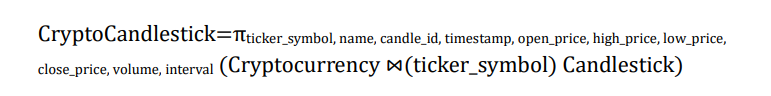
\includegraphics[width=0.8\linewidth]{view3.png}
    \label{fig:placeholder}
\end{figure}

\end{flushleft}





\selectlanguage{greek}

\newpage

\section{Παραδείγματα}

\subsection{Παραδείγματα Πινάκων}

\noindent $\circ$ Παράδειγμα για τον πίνακα \selectlanguage{english}\textbf{User}\selectlanguage{greek} της \selectlanguage{english}CryptfolioDB\selectlanguage{greek}

\selectlanguage{english}

\noindent \begin{tabular}{|l|l|l|l|l|l|l|l|l|}
    \hline
    \textbf{\shortstack{user \\ \_id}} & \textbf{name} & \textbf{email} & \textbf{registered\_at} & \textbf{phone} & \textbf{\shortstack{password\\ \_hash}} & \textbf{salt} & \textbf{\shortstack{last\_pw \\ \_update}} & \textbf{\shortstack{is \\ \_verified} } \\
    \hline
    1 & \shortstack{Aris \\ Dask} & \shortstack{aris@ \\ example.com} & \shortstack{2020-10-25 \\ 09:30:00} & 3069... & \$2b\$12\$xyz... & abc123 & \shortstack{2025-01-01 \\ 09:30:00} & 1 \\
    \hline
    2 & \shortstack{Geo \\ Rouso} & \shortstack{rouso@ \\ example.com} & \shortstack{2023-11-25 \\ 09:35:00} & 3069... & \$2b\$12\$zyx... & def456 & \shortstack{2024-10-25 \\ 09:30:00} & 1 \\
    \hline
    3 & \shortstack{Geo \\ Lav}   & \shortstack{lavlav@ \\ example.com} & \shortstack{2025-09-25 \\ 08:30:00} & 3069... & \$2b\$12\$mno... & ghi789 & \shortstack{2024-10-25 \\ 09:30:00} & 0 \\
    \hline
\end{tabular}

\selectlanguage{greek}
\begin{flushright}
\textit{Εκτίμηση για τον αριθμό των εγγραφών}: $\sim0.5M$\footnote{$M \xrightarrow{} Million$}
\end{flushright}



\bigskip
\noindent $\circ$ Παράδειγμα για τον πίνακα \selectlanguage{english}\textbf{Wallet}\selectlanguage{greek} της \selectlanguage{english}CryptfolioDB\selectlanguage{greek}

\selectlanguage{english}

\noindent \begin{tabular}{|l|l|l|l|l|}
    \hline
    \textbf{wallet\_id} & \textbf{seed\_phrase} & \textbf{cash\_balance} & \textbf{name} & \textbf{type} \\
    \hline
    1 & As7e8w1... & 1500.75 & My Savings Wallet & 1 \\
    \hline
    2 & nd9Cr8q... & 275.50 & Trading Wallet & 1 \\
    \hline
    3 & diwOq9s... & 5000.00 & Investment Team Wallet & 1 \\
    \hline
\end{tabular}

\selectlanguage{greek}
\begin{flushright}
\textit{Εκτίμηση για τον αριθμό των εγγραφών}: $\sim1.5M$
\end{flushright}


\bigskip
\noindent $\circ$ Παράδειγμα για τον πίνακα \selectlanguage{english}\textbf{User \textit{has} Wallet}\selectlanguage{greek} της \selectlanguage{english}CryptfolioDB\selectlanguage{greek}

\selectlanguage{english}

\noindent \begin{tabular}{|l|l|l|l|l|}
    \hline
    \textbf{wallet\_id} & \textbf{user\_id} & \textbf{role} \\
    \hline
    1 & 1 & `owner' \\
    \hline
    2 & 1 & `owner' \\
    \hline
    3 & 2 & `owner' \\
    \hline
    3 & 1 & `member' \\
    \hline
\end{tabular}

\selectlanguage{greek}
\begin{flushright}
\textit{Εκτίμηση για τον αριθμό των εγγραφών}: $\sim2.5M$
\end{flushright}


\bigskip
\noindent $\circ$ Παράδειγμα για τον πίνακα \selectlanguage{english}\textbf{BankAccount}\selectlanguage{greek} της \selectlanguage{english}CryptfolioDB\selectlanguage{greek}

\selectlanguage{english}

\noindent \begin{tabular}{|l|l|l|l|l|l|l|l|}
    \hline
    \textbf{\shortstack{account\\ \_id}} & \textbf{\shortstack{user\\ \_id}} & \textbf{\shortstack{encrypted\\ \_iban}} & \textbf{holder\_name} & \textbf{bank\_name} & \textbf{\shortstack{account \\ \_type}} & \textbf{verified\_at} & \textbf{\shortstack{provider\\ \_token}} \\
    \hline
    1 & 1 & 70s...19  & \shortstack{Aristeidis \\ Daskalopoulos} & AlphaBank & 1 & \shortstack{2023-02-15 \\ 10:30:00} & 123... \\
    \hline
    2 & 2 & 81...00 & \shortstack{Georgios \\ Rousmanis} & PereousBank & 1 & \shortstack{2025-01-20 \\ 09:15:00} & 012... \\
    \hline
    3 & 2 & 98...13 & \shortstack{Georgios \\ Rousmanis} & AlphaBank & 1 & \shortstack{2025-10-20 \\ 09:15:00} & 789... \\
    \hline
    4 & 3 & A7...21 & \shortstack{Georgios \\ Lavdakis} & PereousBank & 2 & NULL &   NULL \\
    \hline
\end{tabular}

\selectlanguage{greek}
\begin{flushright}
\textit{Εκτίμηση για τον αριθμό των εγγραφών}: $\sim0.75M$
\end{flushright}



\bigskip
\noindent $\circ$ Παράδειγμα για τον πίνακα \selectlanguage{english}\textbf{WalletBankTransfer}\selectlanguage{greek} της \selectlanguage{english}CryptfolioDB\selectlanguage{greek}

\selectlanguage{english}

\noindent \begin{tabular}{|l|l|l|l|l|l|l|}
    \hline
    \textbf{transfer\_id} & \textbf{direction} & \textbf{timestamp} & \textbf{amount} & \textbf{wallet\_id} & \textbf{account\_id} \\
    \hline
    1 & `toWallet' & 2024-01-20 09:30:00 & 500.00 & 1 & 1 \\
    \hline
    2 & `toWallet' & 2024-04-20 14:15:00 & 1100.00 & 3 & 2 \\
    \hline
    3 & `toBank' & 2024-05-21 11:45:00 & 1000.00 & 3 & 3 \\
    \hline
    4 & `toWallet' & 2024-05-22 16:20:00 & 75.25 & 3 & 1 \\
    \hline
\end{tabular}

\selectlanguage{greek}
\begin{flushright}
\textit{Εκτίμηση για τον αριθμό των εγγραφών}: $\sim1B$\footnote{$B \xrightarrow{} Billion$}
\end{flushright}


\bigskip
\noindent $\circ$ Παράδειγμα για τον πίνακα \selectlanguage{english}\textbf{Invitation}\selectlanguage{greek} της \selectlanguage{english}CryptfolioDB\selectlanguage{greek}

\selectlanguage{english}

\noindent \begin{tabular}{|l|l|l|l|l|l|l|l|}
    \hline
    \textbf{\shortstack{invitation\\ \_id} } & \textbf{\shortstack{ invitee\\ \_id} } & \textbf{\shortstack{inviter\\ \_id}} & \textbf{\shortstack{wallet\\ \_id}}  & \textbf{status} & \textbf{\shortstack{ invitee\\ \_role}}  & \textbf{expires\_at} & \textbf{created\_at} \\
    \hline
    1 & 1 & 2 & 3 & `accepted' & `member' & \shortstack{2024-01-08 \\ 23:59:00} & \shortstack{2024-01-01 \\ 10:30:00} \\
    \hline
    2 & 3 & 1 & 2 &  `pending' & `viewer' & \shortstack{2025-11-28 \\ 23:59:00} & \shortstack{2025-11-21 \\ 14:15:00} \\
    \hline
\end{tabular}

\selectlanguage{greek}
\begin{flushright}
\textit{Εκτίμηση για τον αριθμό των εγγραφών}: $\sim3M$
\end{flushright}


\bigskip
\noindent $\circ$ Παράδειγμα για τον πίνακα \selectlanguage{english}\textbf{Cryptocurrency}\selectlanguage{greek} της \selectlanguage{english}CryptfolioDB\selectlanguage{greek}

\selectlanguage{english}

\noindent \begin{tabular}{|l|l|l|l|}
    \hline
    \textbf{ticker\_symbol} & \textbf{name} & \textbf{logo\_image} \\
    \hline
    BTC & Bitcoin & 00...1A  \\
    \hline
    ETH & Ethereum & 00...F1  \\
    \hline
    USDT & Tether &  01...BB \\
    \hline
    DOGE & Dogecoin & 01...A1 \\
    \hline
\end{tabular}

\selectlanguage{greek}
\begin{flushright}
\textit{Εκτίμηση για τον αριθμό των εγγραφών}: $\sim10.0M$
\end{flushright}



\bigskip
\noindent $\circ$ Παράδειγμα για τον πίνακα \selectlanguage{english}\textbf{CryptoBalance}\selectlanguage{greek} της \selectlanguage{english}CryptfolioDB\selectlanguage{greek}

\selectlanguage{english}

\noindent \begin{tabular}{|l|l|l|l|}
    \hline
    \textbf{balance\_id} & \textbf{wallet\_id} & \textbf{crypto\_amount} & \textbf{ticker\_symbol} \\
    \hline
    1 & 1 & 0.005000 & BTC \\
    \hline
    2 & 1 & 0.750000 & ETH \\
    \hline
    3 & 1 & 50.500000 & USDT \\
    \hline
    4 & 3 & 2.250000 & ETH  \\
    \hline
    5 & 2 & 0.850000 & BTC  \\
    \hline
\end{tabular}

\selectlanguage{greek}
\begin{flushright}
\textit{Εκτίμηση για τον αριθμό των εγγραφών}: $\sim7.5M$
\end{flushright}


\bigskip
\noindent $\circ$ Παράδειγμα για τον πίνακα \selectlanguage{english}\textbf{Transaction}\selectlanguage{greek} της \selectlanguage{english}CryptfolioDB\selectlanguage{greek}

\selectlanguage{english}
\noindent 
\begin{tabular}{|l|l|l|l|l|l|l|l|l|}
    \hline
    \textbf{\shortstack{transaction \\ \_id}} & \textbf{\shortstack{user \\ \_id}} & \textbf{\shortstack{balance\\ \_id}} & \textbf{amount} & \textbf{\shortstack{transaction \\ \_hash}} & \textbf{\shortstack{price\_at \\ \_timestamp}} & \textbf{timestamp} & \textbf{\shortstack{transaction\\ \_type} } \\
    \hline
    1 & 1 & 1  & 0.50 & 0xa1b... & 45000.00 & \shortstack{2024-05-20 \\ 10:30:00} & `BUY' \\
    \hline
    2 & 2 & 7  & 2.75 & 0xb2c... & 3200.50 & \shortstack{2024-05-20 \\ 10:30:00} & `SELL'  \\
    \hline
    3 & 3 & 3  & 10.0 & 0xc3d4... & 0.45 & \shortstack{2024-05-20 \\ 10:30:00} & `BUY'  \\
    \hline
    4 & 1 & 5  & 5.25 & 0xd4e... & 150.75 & \shortstack{2024-05-20 \\ 10:30:00} & `SELL'  \\
    \hline
    5 & 4 & 5  & 50.0 & 0xe5f6... & 7.20 & \shortstack{2024-05-20 \\ 10:30:00} & `BUY' \\
    \hline
\end{tabular}

\selectlanguage{greek}
\begin{flushright}
\textit{Εκτίμηση για τον αριθμό των εγγραφών}: $\sim10B$
\end{flushright}


\bigskip
\noindent $\circ$ Παράδειγμα για τον πίνακα \selectlanguage{english}\textbf{Candlestick}\selectlanguage{greek} της \selectlanguage{english}CryptfolioDB\selectlanguage{greek}

\selectlanguage{english}
\noindent 
\begin{tabular}{|l|l|l|l|l|l|l|l|}
    \hline
    \textbf{candle\_id} & \textbf{ticker\_symbol} & \textbf{open\_price} & \textbf{high\_price} & \textbf{low\_price} & \textbf{close\_price} & \textbf{volume} & \textbf{interval} \\
    \hline
    CAND001 & BTC & 45000.00 & 45500.50 & 44800.75 & 45200.25 & 1250.50000000 & 1h \\
    \hline
    CAND002 & ETH & 3200.00 & 3250.75 & 3180.25 & 3225.50 & 8500.25000000 & 1h \\
    \hline
    CAND003 & ADA & 0.45 & 0.48 & 0.44 & 0.46 & 500000.00000000 & 4h \\
    \hline
    CAND004 & SOL & 150.00 & 155.75 & 148.50 & 152.25 & 25000.75000000 & 1d \\
    \hline
\end{tabular}

\selectlanguage{greek}
\begin{flushright}
\textit{Εκτίμηση για τον αριθμό των εγγραφών}: $\sim10B$
\end{flushright}


\bigskip
\noindent $\circ$ Παράδειγμα για τον πίνακα \selectlanguage{english}\textbf{CryptoHistory}\selectlanguage{greek} της \selectlanguage{english}CryptfolioDB\selectlanguage{greek}

\selectlanguage{english}
\noindent 
\begin{tabular}{|l|l|l|l|l|}
    \hline
    \textbf{id} & \textbf{ticker\_symbol} & \textbf{current\_price} & \textbf{circulating\_supply} & \textbf{timestamp} \\
    \hline
    CH001 & BTC & 45200.25 & 19400000 & 2024-05-20 10:30:00 \\
    \hline
    CH002 & ETH & 3225.50 & 120000000 & 2024-05-20 10:30:00 \\
    \hline
    CH003 & ADA & 0.46 & 45000000000 & 2024-05-20 11:00:00 \\
    \hline
    CH004 & SOL & 152.25 & 573000000 & 2024-05-20 11:00:00 \\
    \hline
\end{tabular}

\selectlanguage{greek}
\begin{flushright}
\textit{Εκτίμηση για τον αριθμό των εγγραφών}: $\sim10B$
\end{flushright}

\bigskip
\noindent $\circ$ Παράδειγμα για τον πίνακα \selectlanguage{english}\textbf{Alert}\selectlanguage{greek} της \selectlanguage{english}CryptfolioDB\selectlanguage{greek}

\selectlanguage{english}
\noindent 
\begin{tabular}{|l|l|l|l|l|l|l|l|}
    \hline
    \textbf{alert\_id} & \textbf{user\_id} & \textbf{ticker\_symbol} & \textbf{threshold\_price} & \textbf{threshold\_direction} & \textbf{description} & \textbf{is\_active} & \textbf{triggered\_at} \\
    \hline
    ALERT001 & 101 & BTC & 50000.00 & ABOVE & Price above 50k & 1 & NULL \\
    \hline
    ALERT002 & 102 & ETH & 3000.00 & BELOW & Price below 3k & 1 & 2024-05-19 14:30:00 \\
    \hline
    ALERT003 & 103 & ADA & 0.50 & ABOVE & ADA reaches 0.50 & 1 & NULL \\
    \hline
    ALERT004 & 101 & SOL & 200.00 & ABOVE & SOL bullish target & 0 & NULL \\
    \hline
\end{tabular}

\selectlanguage{greek}
\begin{flushright}
\textit{Εκτίμηση για τον αριθμό των εγγραφών}: $\sim10B$
\end{flushright}





\subsection{Παραδείγματα Ερωτημάτων}

\begin{flushleft}

1) \selectlanguage{english}Verified bank accounts \selectlanguage{greek}ενός χρήστη με \selectlanguage{english}user\_id = 2

\begin{figure}[h]
    \centering
    
\includegraphics[width=0.7\linewidth]{query1.png}
    \label{fig:placeholder}
\end{figure}


2) \selectlanguage{greek}Όλες οι αγοραπωλησίες ενός χρήστη με \selectlanguage{english}user\_id = 1

\begin{figure}[h]
    \centering
    
\includegraphics[width=0.7\linewidth]{query2.png}
    \label{fig:placeholder}
\end{figure}

3) \selectlanguage{greek}Όλα τα \selectlanguage{english}pending invitations \selectlanguage{greek}για συγκεκριμένο χρήστη με \selectlanguage{english}invitee\_id = 3

\begin{figure}[h]
    \centering
    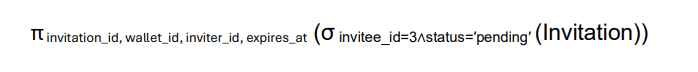
\includegraphics[width=0.7\linewidth]{query3.png}
    \label{fig:placeholder}
\end{figure}

4) Crypto portfolio \selectlanguage{greek}ενός \selectlanguage{english}wallet \selectlanguage{greek}με \selectlanguage{english}wallet\_id = 1

\begin{figure}[h]
    \centering
    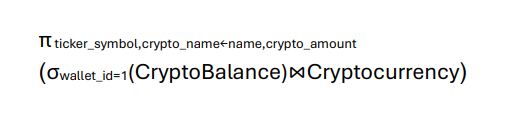
\includegraphics[width=0.7\linewidth]{query4.png}
    \label{fig:placeholder}
\end{figure}


\end{flushleft}


\end{document}


